\documentclass{NSF}
\usepackage{wrapfig}
\usepackage{csquotes}
\graphicspath{{figures/}}
\usepackage{mathptmx}
\Addlcwords{in via for}
\usepackage{xcolor}
\usepackage{fancyhdr}


\begin{document}

% A. Cover Sheet
% A number of the boxes contained on the Cover Sheet are
% electronically pre-filled as part of the FastLane login process
% Complete the rest of your info there

% B. Project Summary
%\title{Sexy HoQ for Autonomy Dynamic Decision}
\newsection{A}
%\section{Physical Human Factors Report: Tristan Griffith}
\rhead{\today}
\begin{center}
{\textbf{\Large Brief on Modal EEG Fingerprinting}}\\
\vspace{2mm}
{\large  Tristan Griffith}\\
\vspace{2mm}
{\large Dr. James Hubbard Jr.}
\noindent\rule{\textwidth}{2pt}
\end{center}

%\begin{wrapfigure}{r}{0.45\textwidth}
%\centering
%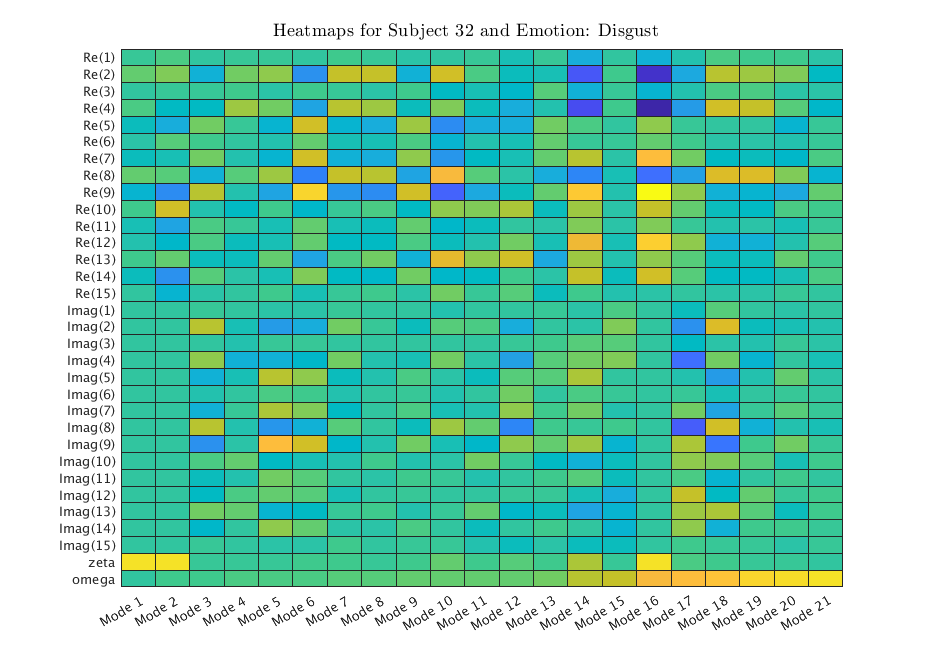
\includegraphics[scale=.3]{../../../figures/demo_map.png} 
%\caption{Modal Heatmap for Subject 32}
%\end{wrapfigure}
We postulate that data driven system identification methods of EEG data, such as Output Only Modal Analysis and Dynamic Mode Decomposition, may yield predictive models of cognition for more complete information flow between human operators and co-robots. As an initial step to verify that there is statistically significant information in these modal representations, an artificial neural network is proposed to discriminate subjects in a database. If the network shows sufficient accuracy in identifying subjects from the modal representation of their brain activity, we gain confidence that the modal representation is capturing significant information in the modes. It is shown that the network can discriminate 32 subjects from one another with $>$99\% accuracy based on knowledge of the significant modes alone.\


Output Only Modal Analysis (OMA) algorithms have been in use since at least the 90's. Originally developed for large mechanical structures, which are extremely difficult to precisely excite, OMA algorithms assume broadband stochastic input to the system in order to determine a state space model for a given system. The specific method applied to this data results from solving a set of linear equations with least squares to match data held in a Hankel matrix. When applied to the DEAP dataset, 21 significant complex modes are determined, which may be represented as a heatmap.\

\begin{wrapfigure}{r}{0.6\textwidth}
\centering
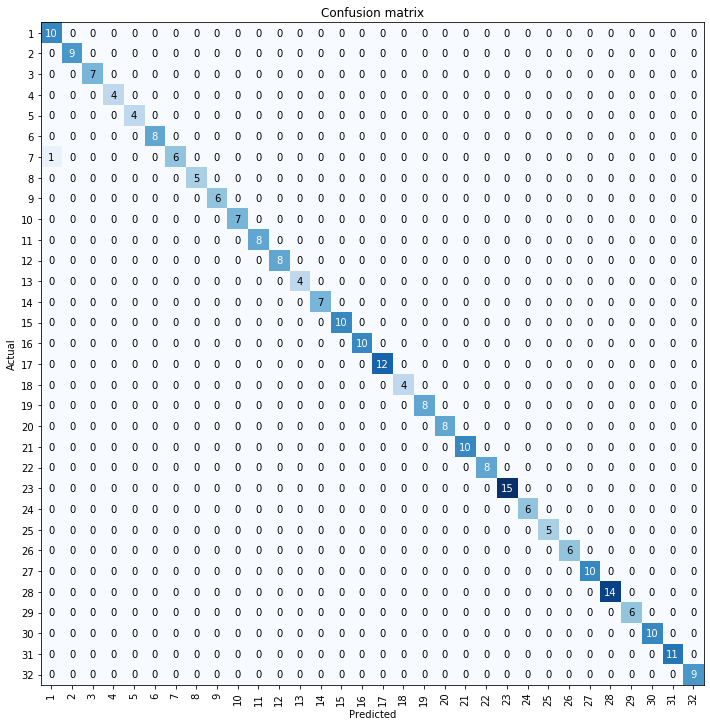
\includegraphics[scale=0.4]{../../../figures/conf_mat.png}  
\caption{Confusion Matrix for Neural Net}
\end{wrapfigure}
Having generated modal heatmaps for each of the 40 one minute trials across 32 subjects, 1280 modal heatmaps are generated. 1024 of these heatmaps are shown to the neural network, along with the subject label 1-32. The remaining 256 heatmaps are reserved for validation, without the subject label. Using a simple ResNet18 architecture, the network can distinguish subjects from unseen heatmaps with an accuracy of 99\% with less than 10 minutes of total training time. The relevant confusion matrix is included. Note that over all 256 unseen images, the network has only made one mistake, confusing subjects 1 and 7. This suggests that there is statistically significant information contained in the identified modes.




%\begin{displayquote}
%The class of monotone DNF expressions is learnable via an algorithm $B$ that uses $L=L(h,d)$ calls of examples and $dt$ calls of oracle, where $d$ is the degree of the DNF expression $f$ to be learnt and $t$ the number of variables.
%\end{displayquote}


%\begin{wrapfigure}{r}{0.55\textwidth}
%\centering
%\includegraphics[scale=.5]{../figures/complexity.png} 
%\caption{The Error-Complexity Trade Off}
%\end{wrapfigure}



% C. Table of Contents 
% A Table of Contents is automatically generated for the proposal by FastLane

% D. Project Description
%\newpage\newsection{D}
%\section{Project Description}
\subsection{Introduction}
Rapid development of autonomous technology has led to premature deployment, putting drivers, pedestrians, and companies at risk.  Recent accidents have shifted the narrative on autonomous vehicles, with many calling for a reevaluation of expectations 
\cite{Wakabayashi2019,Dickson2019,Higgins2019}.
Yet, there is a proliferation of research activity in the field. New tools and techniques for automation of vehicles are being developed with applications across the spectrum of industry, academia and government. Autonomous features are now available in modern automobiles that allow them to automatically park, maintain tracking within a lane, and control speed in conformance with traffic. These features require that the vehicle maintain a certain degree of
\textbf{situational awareness} of the environment that they operate in. In this regard there have also been significant advances in sensor technology and sensor fusion techniques that merge data gathered from Lidar, Radar, Low Light cameras and acoustic sensors mounted on board the platform
\cite{Liu2018,Ingrand2017}.
As the research community pushes toward full autonomy, additional sensing capability that includes road and sign sensors, weather and traffic data have been explored in a concept called \textbf{connected autonomy} to give the vehicle as much information as possible, about its operational environment, so that it can make informed decisions, using artificial intelligence in-situ, to improve safety and operational trust.\\

Autonomous systems are indeed engineered to unburden the operator of awareness over the vehicle's safety processes. While autonomous engineering is designed to appeal to the purchaser, it effectively relieves the operator of an essential duty; to remain cognitively engaged during operation of the system. In reality, many of the systems engineered into the vehicle actually diminish the driver's capacity to remain engaged \cite{Cunningham2015}. This is known as 
\textbf{engineered distraction} in the industry. Coupled with devices, e.g. the cell phone, a very disengaging driving environment arises.\\

Autonomous systems require the interoperability of real-time sensors that calculate environment perception, planning, and vehicle control. While autonomous systems move forward, addressing the cognitive engagement of the driver has been quite overlooked even though it is vitally important \cite{Kaber2017}. This is necessary in urban areas where traffic is heavier and more unpredictable than roadways where unexpected road or driving conditions occur less frequently. Current approaches generally do not consider the human operator's role as a critical component of the autonomous system. These approaches generally do not consider the human's role as a critical component of the autonomous system. Even though manufacturers tout the accuracy and safety of their respective autonomous systems, fatalities have occurred \cite{NTSB2017}.\\

Ultimately the research proposed herein will help to avoid anticipated breakdowns in human performance and situational awareness during autonomous driving. A variety of public safety challenges emerge from the increase of autonomous vehicles, having an annual projected market growth of 40\% between 2019-2026 \cite{Kumar2018}. Despite the projected expansion of autonomous vehicles in the very near future, training of human operators (especially elderly populations) is scarce and hard to scale. The proposed work is both timely and relevant since it can warn drivers in a passive and automated way regarding loss of their situational awareness, helping them avoid accidents and promoting public safety in various types of high-risk scenarios.

\subsection{Objectives}
The following is a concise statement of the proposed program objectives:\
\begin{enumerate}
  \item Develop an engineering approach to cognition that provides a rigorous robust structure to determining human cognitive states. 
  \item Develop and apply tools and techniques using a state-based approach that allows researchers to design in a well understood mathematical structure using readily available tools and techniques. This will result in an ability to determine the mental state of human operator for improved situational awareness will also allow more efficient "teaming" between machines and humans to successfully meet system mission goals. 
  \item Apply a Quantum-like theoretic approach that informs a methodology that can consistently approach the notion of contextuality, between any combination of human cognitive states and system operational environments. We believe that the mathematics of quantum theory is potentially relevant to all the contextual phenomena such as trust.
\end{enumerate}



\subsection{Rational and Scope}
\subsubsection{The Autonomy Conundrum}
As researchers and manufacturers move rapidly toward achieving full autonomy, human operators and passengers are becoming increasingly disconnected. As the vehicle situation awareness increases, so concomitantly does the human situational awareness decrease \cite{Flemisch2003}. Lower situational awareness of human operators means they are less likely to efficiently take over manual control when needed if an anomaly occurs. Mica Endsley defines this as the 
\textbf{Autonomy Conundrum} and points out in her paper "From Here to Autonomy", that the goal of full system autonomy is quite difficult, and most systems will exist at some level of semi-autonomy in the foreseen future \cite{Endsley2017}. Thus, the automation conundrum potentially creates a fundamental barrier to autonomy in safety critical systems, such as driving. While recent system autonomy efforts are beginning to leverage artificial intelligence and learning algorithms to allow the platforms to better adapt to unanticipated and changing situations; it is becoming clear that the design and inclusion of human-autonomy interfaces are needed. There has been much research demonstrating how humans have fared poorly with increased automation and results in automation complacency, over reliance on automation, loss of situational awareness and spatial orientation, and skill loss \cite{Schutte2017,Gouraud2018,Parasuraman1993}. These have contributed to human errors, accidents and loss of trust.\\

Modern autonomous systems are, and will be in the future, dependent on the development of successful approaches to human–autonomy teaming. Here we define "the system" as consisting of the platform, the software and the human "operator". Future automation should be designed to mitigate the risk associated with the autonomy conundrum by actively assessing and managing the humans' engagement. The philosophy behind this approach, which is embraced here, is that the human's primary role is to step in and deal with emergencies, non-normals, and unanticipated situations. The system should be designed to keep the human in proper condition to intervene and take over when necessary.

\subsubsection{Human Cognition and Engagement}
When humans are acting as passive monitors of autonomous driving, it is inherently difficult for them to fully understand what is going on due to lower levels of \textbf{cognitive engagement}. Here we propose to investigate and monitor the features that influence the human cognitive processes involved in successful oversight, intervention, and interaction with automated systems.  Unexpected automation transitions will occur when the automation suddenly passes control to the human operator, who cognitively may not be ready to take over. This means that in addition to situational awareness of the environment, the vehicle also requires situational awareness of the human as well. This demands a real time assessment of human cognition. We note the difference between discrete cognitive tasks associated with human intervention which requires more conscious attention sporadically, as compared with continuous manual control, which generally requires lower attention over an extended period \cite{Endsley2017}.\\

Maintaining vigilance for discrete interventions can be quite challenging because attention may be redirected to competing tasks. NASA has developed an effective \textbf{Cognitive Engagement Index} for determining the level of task engagement by pilots executing various task in the cockpit during flight \cite{Hart1988}. Through a series of empirical studies, they correlated pilot engagement with EEG measurements of brain waves. They formed an engagement index, using real time monitored brain waves ($\beta,\alpha$), which was calculated and found to correlate well with observed pilot engagement \cite{Matthews2015,Cao2009}.

\subsubsection{Brain Waves as Cognitive Indicators}
The brain has nerve cells that fire electrical signals day and night, forming distinctive arrangements called brainwave patterns. These highly unique patterns are closely connected to our thoughts, emotions, moods, and biological chemistry, everything we do \cite{LopesdaSilva1991}. The electrical oscillations which we call brain waves were first discovered using electroencephalogram (EEG) techniques, which involve placing electrodes on the scalp. Researchers have noted activity over a range of different frequencies, from delta (0.5 to 4 hertz) through gamma (25 to 140 Hz) waves \cite{Klimesch,Kaufman1992,Buzsaki1994,Yamamoto1990}. 
The slowest occur during deep sleep, with increasing frequency associated with increasing levels of consciousness and concentration. Brain waves are relevant to behavior, and are an important mechanism that contributes to memory, perception, attention and even consciousness \cite{Miller1991,Fernandez1995}.\\

Human cognition and emotion are very difficult to determine just by looking at the face and the behavior of a person. There has been considerable research conducted to identify human emotion via the study of brain waves. The relevant mental states of human drivers may include, drowsiness, fatigue and distraction. Here we propose to use modern, non-invasive brain wave monitoring technology and quantum theory to determine, in real time, the mental state of human operators in autonomous self-driving vehicles.
	\begin{figure}[h]
    \centering
    \includegraphics[scale=.8]{../figures/fig1.jpg} 
    \caption{Typical Brain Wave Time Histories}
    \end{figure}
This will provide the vehicle with the needed situational awareness of the human to mitigate the existing automation conundrum. In this manner the vehicle can be capable of transmitting haptic cues (such as pulses and vibrations) to signal an anticipated need for human engagement.

\subsubsection{Quantum Cognition: An Engineering Approach}
The general mathematical structure of quantum theory provides us with an engineering approach to cognition that is not only applicable to physics but to any scientific domain that has a need to formalize uncertainty and probability and can be formally applied to human cognition.  Quantum theory provides us with a methodology that can consistently convey the notion of contextuality between any combination of autonomous system components and operational environments \cite{Kitto2013}.\\

We believe that the mathematics of quantum theory are potentially also relevant to the contextual phenomena of trust. We note that in applying the mathematical machinery of quantum theory to human cognition we do not wish to imply that the human brain and the corresponding psychological processes have a quantum nature. We simply wish to take a quantum-like modeling approach to assessing human cognition by defining the state of the human in a geometrical fashion using state vectors placed in a specific basis. Then context can be modeled to a great extent. In the quantum approach, context is much more than just a simple label and change of context can occur by changing the basis with a unitary transformation operator. Here we are simply using the mathematics of quantum theory as a tool to better describe and explain the human cognitive state.  These are all tools quite familiar to engineers.

\subsubsection{Brain Waves and the Quantum Probability}
From a Quantum viewpoint, all the above-mentioned brainwave frequencies are normally present simultaneously in the brain. Researchers, however, often refer to the dominant frequency in the EEG pattern as what determines the current state of the brain, i.e. the cognitive state \cite{Aufenberg2005}. If for example the amplitude of the alpha range frequencies is highest, then the brain is said to be in the alpha stage. Note, that other frequencies still exist, and it is impossible to give any "exact frequency your brain is operating on." However, for simplification purposes, it is often assumed that such a single frequency exists. This paradox can be addressed by Quantum theory for a better determination of brain cognition.\\

Many wearable devices can track your heart rate, steps, body temperature or sleep, but recently there has emerged a new class of wearables aiming to move beyond tracking the physical to tracking the mind. The makers of these "brain wearables" — which come in the form of headsets with electrodes — claim the devices can improve your focus, detect stress and even let you play video games with your brain \cite{muse,emotiv}. The devices work by detecting the brain's electrical activity, or brain waves, using electroencephalography (EEG). EEG signals are related to concentration, memory, attention and even thoughts about moving different parts of the body. More relevantly, the company Freer Logic has teamed with autonomous car makers to create an award-winning car seat headrest that provides real-time brain wave data without contacting the vehicle's driver. The current range of the brain wave measuring device is from 6 to 10 inches from the head. It is currently in development via automotive OEM and Tier 1 suppliers in an effort to determine fatigue, drowsiness, cognitive load, distraction, stress, and relaxation.
	\begin{figure}[h]
    \centering
    \includegraphics[scale=1.0]{../figures/freer_logic.jpg} 
    \caption{Freer Logic's Award-Winning Neurobiomonitor Headrest}
    \end{figure}
It is a common belief among neuro scientist that there are six basic emotions consisting of happiness, sadness, fear, anger, surprise and disgust \cite{Batty2003,Eimer2003}. This suggest that the states shown in Figure 2 can be represented as a weighted, linear combination of these six basic emotional states. In our Quantum like approach to cognition taken here, these can be represented in terms of a fundamental basis set in Hilbert space \cite{Ashtiani2015}. This is because Quantum Probability (QP) theory, is a geometric theory of assigning probabilities to outcomes. A vector space (called a Hilbert space) is defined, in which possible outcomes are represented as subspaces of this vector space. When we ask questions about human cognition and seek outcomes this informs the technical QP terms observables and propositions. The vector space represents all possible outcomes for questions we could ask about a system of interest. Here the system we consider is a hypothetical person and the general question of that person's emotional state. Then, one-dimensional subspaces (called rays) in the vector space would correspond to the most elementary emotions possible, e.g. happiness, sadness, fear, anger, surprise and disgust. The number of unique elementary emotions and their relation to each other determine the overall dimensionality of the vector space. More general emotions, such as relaxation, would be represented by subspaces of higher dimensionality. The details of our proposed technical approach are presented in what follows.

\subsection{Proposed Research}
\subsubsection{A Quantum Engagement Model}
To clarify our approach, we have formulated a very simple version of the quantum probability approach to cognition: Engaged-Unengaged. This is the most basic form of situational awareness for an operator. Quantum Probability theory is a geometric theory of assigning probabilities to outcomes. The use of a quantum probability approach to human cognition is currently developing, good introductions to the broad area of Quantum Probability applications can be found in many texts \cite{Busemeyer2012,Khrennikov2003,Schwartz2005}. Many cognition issues do not fit into a standard probability description, but quantum probability and decision theory are beginning to resolve these difficulties \cite{Ashtiani2015,Yukalov1998}. A more detailed theoretical summary of quantum probability theory will be given later in this proposal; in this section we will make use of the basic ideas. The Engaged-Unengaged model discussed in this section is very similar to the Quantum Spin model that illustrates the quantum probability theory section. Note that we are not saying that the human brain is described by a microscopic atomic-level quantum mechanics. We mean that the brain in cognition behaves in a quantum-like way that can be analytically described by quantum probability theory \cite{Blutner}.\\

A Hilbert space (which is a vector space with an inner product) is defined, in which possible outcomes are represented as subspaces of this vector space. The Hilbert space represents all possible outcomes for questions we could ask about a system of interest. Here we consider a hypothetical person and the general question of that person's emotional state. Then, one-dimensional subspaces (called rays) in the vector space would correspond to the most elementary emotions possible, e.g. anxiety, stress, distraction, fatigue. The generators of these one-dimensional subspaces are the basis vectors for the Hilbert Space. The number of unique elementary emotions and their relation to each other determine the overall dimensionality of the vector space; the primary emotional states are taken to be orthogonal vectors in the Hilbert space.  More general emotions, such as happiness, could be represented by subspaces of higher dimensionality. In quantum probability theory, it is easier to keep track of the (orthogonal) projections onto the primary emotional subspaces and to manipulate these projections as linear operators on the Hilbert Space. One of the most attractive properties of quantum probability theory over standard probability theory is the use of the projections to handle sequences of events or the conditioning of events by other events; this is done by simply multiplying projection operators.\\

Because the Hilbert Space has linear operations where addition and (complex) scalar multiplication can take place, the general state of the human operator can be seen as linear combinations of these \textbf{basic emotional states}. For a simple Engagement model, there are only two basic emotional states: $\phi_1\equiv $Engaged and $\phi_2\equiv$ Unengaged. All other emotions in this model are \textbf{mixed states} and will be linear combinations of these two orthogonal states: $x=\alpha \phi_1+\beta \phi_2$ where $\alpha$ and $\beta$ are complex numbers. The squares of the magnitudes of these scalers are the probabilities of being in each of the basic states: $|\alpha|^2=$probability of being fully engaged and $|\beta|^2=$probability of being fully unengaged, and these probabilities must add up to one ($|\beta|^2+|\alpha|^2=1$) which is the total probability in the Engagement  quantum probability space. Consequently, all the mixed states will be vectors that lie on the surface of a unit ball or in this simple case on a circle. The orthogonal projections will resolve these mixed states into the vector components $P_1x=\alpha \phi_1$ and $P_2x=\beta \phi_1$ in each basic emotional subspace. These projections are the basic \textbf{quantum observables}.
	\begin{figure}[h]
    \centering
    \includegraphics[scale=1]{../figures/fig3.jpg}  
    \caption{A Low-Dimension Representation of Quantum State}
    \end{figure}
Therefore, in this simple engagement model the human operator could be in \textbf{any} mixed state on the surface of the circle. Continuous measurements of mixed quantum states that can reveal and distinguish the basic emotional states are possible. There is already evidence that the elementary human emotions can be identified and that their number is small \cite{Ekman1992,Celeghin2017}, and that quantum probabilistic structure appears in human cognition \cite{Aerts2011}. Furthermore, brainwaves (EEG) may be used to detect and measure and identify these basic emotional states \cite{Heraz2007,Deng2010,Basar1999}.

\subsubsection{Quantum Dynamics and the Quantum Kalman Filter}
Our approach to the measurement problem will be a Quantum Kalman filter that uses the human emotions as states from a quantum-like system and the EEG brainwaves as measured outputs due to linear combinations of these basic states. The quantum filter would then be used to distinguish and recover estimates of the basic states from the brainwaves. Quantum Kalman Filtering and Estimation Theory has begun to be developed \cite{Accardi2003,Bouten2009}.\\

For a Quantum Kalman Filter to work, the dynamic behavior of the states is required. It is from this dynamic behavior and the experimental measurements that the human emotions could be reconstructed. The description of Quantum Dynamics is contained in the Schrodinger Wave Equation: 
\begin{equation}
i \hbar \frac{\delta x}{\delta t}=Hx\\
\end{equation}
\begin{equation}
x(0)=x_0
\end{equation}
Where the observable operator   is the Hamiltonian Energy operator for the quantum system of interest. The Planck constant is not significant in cognition and can be set equal to 1 
For the simple Engagement Model this Hamiltonian has the form: 
\begin{equation}
H=\sum_{k=1}^2 \lambda_k P_k=\lambda_1 P_1+ \lambda_2 P_2
\end{equation}
Where the Projections are onto the engaged and unengaged subspaces.The wave solution is
\begin{equation}
x(t)=U(t)x_0=e^{-i\frac{H}{\hbar}t}x_0=\sum_{k=1}^{2} e^{-i\frac{H}{\hbar}t} P_k x_0
\end{equation}
This generates a unitary group $H$ which maintains the wave solution state on the surface of the unit ball (in our example the boundary of the unit circle).  This means that mixed states just rotate on the unit circle while their overall probability remains one. From this dynamical description, the Quantum Kalman Filter must recover estimates of the mixed states as combinations of the individual basic emotional states of engaged and unengaged from measurements of brainwaves:
\begin{equation}
i \hbar \frac{\delta \hat{x}}{\delta t}=H \hat{x}+K(y-\hat{y})\\
\end{equation}
\begin{equation}
\hat{y}=Cx
\end{equation}
\begin{equation}
x(0)=x_0
\end{equation}
To verify this filter as a quantum measurement system working on brainwaves, we propose to use the current \textbf{Engagement Index}. This was developed by Dr. Alan Pope of NASA Langley who created the only known successful algorithm to measure "Engagement" and used it to study cognition of pilots in the cockpit of airplanes \cite{Pope1995}  . The Engagement Index = Beta Power/(Alpha Power + Theta Power). It appears to be the most reliable index found to date. But the index was developed empirically without any attempt to derive it from a theoretical basis. We would develop the index as an observable from our quantum probability approach. We propose to develop other cognitive metrics, for the basic emotions describe earlier, along with additional indices in order to apply the Quantum Theory.

\subsection{Project Participants}
\textbf{Dr. Chaspari's} research focuses on the computational study of \textbf{human behavior}. She has worked on knowledge-driven models of physiological signals to capture human behavior in real-life through sensory-based devices and has applied these to mental and physical well-being applications relevant to health and education. Her work includes the development of personalized and population-specific models that integrate person-dependent characteristics in order to provide reliable descriptors of human behavior, as well as the development of transfer learning techniques to mitigate the problem of data sparsity for human-related applications. Findings from her work have benefited the domains of family studies through the prediction of interpersonal conflict between romantic partners, diabetes monitoring through the estimation of meal composition, as well as education through the development of personalized automated feedback for reducing public speaking anxiety. Dr. Chaspari is the founder and Director of the HUman Bio-Behavioral Signals (HUBBS) Lab which will be used in this research effort.\\

\textbf{Dr. Hubbard} is a member of the National Academy of Engineering with more than 30 years of experience in \textbf{haptic sensing}, adaptive structures, system design and distributed parameter systems. He has developed novel techniques for structural shape control that involve complex system design in \textbf{Hilbert space}. Specific to this effort he has develop a smart automotive seat that will be used to monitor the occupant’s activities. He has more than 2 dozen patents that span the applications of medical, automotive, photonics and structural control. He is internationally known for his work in adaptive structures and is widely recognized as one of the founding fathers of the field. He is a Fellow of the AIAA and ASME. Dr. Hubbard is founder and Co-Director of both the Rellis Starlab Facility and the Morpheus lab which will be used in this research effort.\\

\textbf{Dr. Balas} is the Jack D. Whitfield Professor of Dynamical Systems and the Director of the Center for Autonomous and Evolving Systems at the University of Tennessee Space Institute. He was formerly a distinguished faculty member in Aerospace Engineering at Embry-Riddle Aeronautical University, and formerly the Guthrie Nicholson Professor of Electrical Engineering and former Head of the Electrical and Computer Engineering Department at the University of Wyoming. He has the following technical degrees: PhD in Mathematics, MS Electrical Engineering, MA Mathematics, and BS Electrical Engineering. He has held various positions in industry, academia, and government. Among his careers, he has been a university professor for over 40 years with RPI, MIT, University of Colorado-Boulder, University of Wyoming, and Embry-Riddle Aeronautical University and has mentored 44 doctoral students to completion of their degrees. He has over 350 publications in archive journals, refereed conference proceedings and technical book chapters. He has been visiting faculty with the Institute for Quantum Information and the Control and Dynamics Division at the California Institute of Technology, the US Air Force Research Laboratory-Kirtland AFB, the NASA-Jet Propulsion Laboratory, the NASA Ames Research Center, and was the Associate Director of the University of Wyoming Wind Energy Research Center and adjunct faculty with the School of Energy Resources. He is a life fellow of the American Institute of Aeronautics and Astronautics (AIAA), a life fellow of the Institute of Electrical and Electronic Engineers (IEEE), and a fellow of the American Society of Mechanical Engineers (ASME). He is the recipient of the AIAA GNC Control Systems Heritage award for 2018.\\

\textbf{Freer Logic, Inc.} has been in the field of neurocybernetics for nearly 30 years. It has five patents in the advancement of neurotechnology. Freer Logic will supply equipment and support to the project. Freer Logic also has access to neurotechnology experts who can assist with testing protocols, data analysis, and facilities. Freer Logic's will support this program with its award winning Neurobiomonitor headrest which provides real-time brain data without contacting the vehicle's driver. Current range is from 6 to 10 inches from the head. It is in development via automotive OEM and Tier 1 suppliers to determine fatigue, drowsiness, cognitive load, distraction, emotion, stress, and relaxation.

\subsection{Research Management Plan}
\subsubsection{Sampling Methods and Protocols}
The proposed work will develop data collection protocols to evaluate situational awareness under various mental states. The mental states of interest are guided by previous literature, are of high relevance to driving scenarios, and include fatigue/drowsiness, distraction, and cognitive load \cite{Healey2005,Funfgeld2016,Yang2017}.Situational awareness will be evaluated under three distinct conditions of increasing complexity: a constrained laboratory setting (Phase 1), a simulated driving condition (Phase 2), and a real-life driving condition (Phase 3). Participants' inclusion criteria will include the drivers being above 18-years old, having a valid driver's license, and taking no medication that could affect their driving aptitude.\\
\textbf{Phase 1: Constrained testing protocol to elicit driver's states}\\
The Test of Variables of Attention (T.O.V.A.), a continuous performance designed to test sustained attention and impulse control to a continuous activity, will be assigned to participants. T.O.V.A is theoretically grounded on psychological research \cite{Leark1997} and will provide a constrained well-defined in-lab testing experience to estimate participants' situational awareness and their corresponding neurophysiological reactions. It includes a simple computer game of total duration of 21.6 minutes and incorporates several stimuli. Participants have to detect two target paradigms, a frequent and an infrequent stimulus, presented among others in a pre-determined occurrence ratio (3.5:1 targets to non-targets). Evaluation criteria will include target omission, commission, response time, and response variability.\\
\textbf{Phase 2: Simulation of driving experience}   \\
Participants will be instructed to sit in the driver's seat in a simulated environment while the autonomous vehicle is driving in various simulated environments (rural, urban, freeway) and intervene only when they have to. The target mental states will be elicited as shown in Table 1. Self-reported measures obtained in the beginning and end of the session will be further used in order to get a complete view of a participant's mental state. Each mental state will be separately examined in order to better understand its individual contribution to neurophysiological changes. Neurophysiological signals of peripheral physiology and brain activity (e.g., electroencephalogram, electrocardiogram, electrodermal activity) will be collected while the participants are driving.\\
\begin{table}[]
\centering
\caption{Elicitation Methods of Mental States of Interest}
\begin{tabular}{||c c c||}
\hline
Mental State   & Neutral Condition                                                                                                                      & Elicitation Method                                                                                                                                                                                                     \\ \hline
Fatigue        & \begin{tabular}[c]{@{}l@{}}Participants will be asked \\ to have a full night sleep ($\sim$8 hrs)\\ before the experiment\end{tabular} & \begin{tabular}[c]{@{}l@{}}Participants will be asked to\\ come in early in the morning\\ ($\sim$4 hrs sleep).\end{tabular}                                                                                            \\ \hline
Distraction    & \begin{tabular}[c]{@{}l@{}}No distractions present inside the \\  vehicle.\end{tabular}                                                 & \begin{tabular}[c]{@{}l@{}}Participants will be given a\\ smart device and they will\\ be allowed to use it \\ (e.g. text, talk, view videos).\end{tabular}                                                \\ \hline
Cognitive Load & \begin{tabular}[c]{@{}l@{}}No outside stimuli to challenge\\ participants cognitive load\end{tabular}                                  & \begin{tabular}[c]{@{}l@{}}Participants will be given a \\ simulation scenario with \\ challenging driving conditions \\ (e.g. crowded intersections,\\ adverse weather, rapidly\\ approaching vehicles).\end{tabular} \\ \hline
\end{tabular}
\end{table}
\textbf{Phase 3: Real-world driving experience}
According to this last experimental setting, participants will be asked to sit in an autonomous vehicle that will take them through a pre-determined route in the RELLIS campus of Texas A\&M, a high-class research facility designed to accommodate controlled autonomous driving experiments. At the Rellis Starlab Facility participants will be given a roadmap of the route and will be instructed to intervene if any unexpected adverse events come up. A co-driver will accompany the participants at all times and will be able to intervene at any given moment to ensure participants' safety and mitigate hazardous factors. Participants' mental states will be elicited as in the simulated experiments (see Table 1) and neurophysiological signals will be recorded at all times. Cameras will be placed inside and outside the vehicle to obtain situational information relative to environmental factors.
\subsection{Available Facilities}
\subsubsection{Rellis Starlab Facility}
The Rellis Starlab Facility is part of a 2,000-acre RELLIS campus which promotes advanced research and technology development and education. Through the RELLIS Starlab Facility, academic, government and industry partners, along with Texas A\&M students, faculty, staff collaborate to find innovative solutions to pressing engineering and technology challenges that affect the community, the state of Texas, the nation, and ultimately, the world. The expansive campus provides the facility with both high-fidelity indoor simulation and training as well as outdoor testing, validation, and verification of software algorithms. The extensive indoor and outdoor capabilities combine to do hardware-in-the-loop tests. These are complemented with state-of-the-art equipment for all types of modeling, simulation, and testing.
\subsubsection{HUman Bio-Behavioral Signals (HUBBS) Lab}
HUman Bio-Behavioral Signals (HUBBS) Lab focuses on the integrated computational study of physical well-being and human behavior through the use of both overt behavioral signal information (e.g. speech, language) and covert biomarkers (e.g. biomedical signals) as well as systems theoretic modeling of human interaction. The long-term goal is to integrate the data-scientific and context-rich bio-behavioral approaches towards novel individualized diagnostic, rehabilitation, and intervention tools including human-assistive bio-feedback systems for empowering well-being, health, and defense applications.
\subsubsection{Morpheus Lab}
Morpheus Lab at Texas A\&M University focuses on smart materials and human-robot teaming. The existing equipment in this facility is well suited to the task. NADS compatible driving simulators, custom adaptive sensors, and virtual reality devices couple for measurement of dynamics in human systems. Among these is a full motion capture facility.  
\subsubsection{Unmanned Systems Lab}
Unmanned Systems Lab conducts research which focuses on Mapping, Localization, Guidance, Navigation and Control for developing autonomous ground and aerial vehicles. Our projects span from algorithmic design and implementation to field experimentation of aerial and ground robots.  A specific goal is field deployment of such vehicles in relevant environments. They are routinely deploying autonomous shuttles on campus, self-driving cars, trucks and Unmanned Aerial Vehicles (UAVs). These assets are part of the Rellis Starlab Facility and include self-Driving shuttles that will be used in this effort.

\subsection{Project Schedule}
The project exists in three distinct phases as described above. Each phase is contained in a single calendar year.
	\begin{figure}[h!]
    \centering
    \includegraphics[scale=0.7]{../figures/schedule2.PNG}       
    \caption{Project Timeline}
    \end{figure}
\subsection{Anticipated Future Results}
A fully established quantum architecture for human state detection in autonomous ground vehicles is expected. The performance of this architecture is expected to exceed that of established camera-based systems. As discussed above, this real time architecture shall describe driver states of interest. It is difficult to precisely define what these fundamental states may be at present, which is another expected insight of the work. An exciting consequence of this architecture is the ability to modulate driver state through change of context. Understanding of stimuli that successfully collapse the quantum vector to a desired state is also expected. During the final phase of development, the architecture will see real world deployment, making it unique among other quantum models. All results will be well documented and publicly available.
\subsection{Contribution to Education}
\subsubsection{Quantum Lecture Series}
The J. Mike Walker '66 Department of Mechanical Engineering is well established as a cultivator of distinguished visiting lectures. The PI proposes to leverage this series to bridge the gap between quantum modeling and engineering, as both groups have different verbiage. Quantum approaches will become increasingly relevant as computing capabilities increase, and it is crucial that engineers and educators be prepared to use this technology. By hosting top minds in quantum cognition and engineering, the PI can begin to establish a unique environment encouraging further growth of quantum modeling in engineering.
\subsubsection{Strive to Increase Involvement of Underrepresented Students}
The College of Engineering at Texas A\&M University has identified strategies to "expand outreach and recruiting programs to diverse populations" as a key topic for its 2017-2025 strategic plan. As a result, resources are available to involve both undergraduate and high school students in this area of research. The PI proposes summer internships for high school students, as well as regular lab support from undergraduate students, with a strong commitment to mentorship and outreach for underrepresented students. Students will be exposed to an existing diverse research environment, as well as technical challenges in programming, data collection, and machine learning.
\subsubsection{Develop New Curriculum at Texas A\&M University}
In addition to exploration of the research topics above, the PI proposes development of a new graduate course on Quantum Information Systems and Quantum Control to foster growth of the field. There are many potential applications for these quantum models, and the addition of a new course will encourage students to create new solutions to current problems. 
\subsection{Intellectual Merit and Broader Impacts}
\subsubsection{A Unique Approach}
There have been many efforts to monitor human state with sensors and machine learning. The quantum solution outlined above is a new and creative approach to the autonomy conundrum. Quantum cognitive models have been developed, but not applied. Others have applied sensors and machine learning as a broad solution. The application of a quantum-like approach to human state detection is undeveloped and has broad impact. The work has potential to advance knowledge in quantum cognitive systems and human-robot teaming. The proposed team includes the foremost experts on infinite dimensional systems, quantum control, and biofeedback tools. The team is inspired by the seemingly quantum-like nature of human behavior and seeks to develop quantum modeling techniques.
\subsubsection{A Solution to the Autonomy Conundrum}
The automation conundrum will undermine performance and safety in many applications. New methods for increasing shared situational awareness are paramount to unlocking the economic, societal, and environmental benefits of autonomy, and are accordingly of interest to academic, government, and industrial organizations. Every day such methods are not in development, manufacturers continue to release underdeveloped solutions. These autonomous features cost dollars, public opinion, and lives. Research that, as outlined in this proposal, actively seeks out solutions to the autonomy conundrum is the only way to move the field forward. Fully autonomous systems are impossible until a solution exists. The proposed research offers an exploration of a direct solution to this challenge, and solutions will be well documented and freely available to the public. 
\subsubsection{Advancement of NSF's 10 Big Ideas}
NSF’s 10 big ideas support the long-term prosperity of the nation, through advancement of critical fields. Quantum computing is key to information processing in the 21st century. While the proposed research is not quantum in a traditional sense, it encourages the creative application of quantum principles borrowed from physics. This idea strongly correlates with \textbf{Growing Convergence} Research as identified by NSF. Further, the PI argues that the topic falls well within the theme of building human-technology partnerships as described in the \textbf{Future of Work} core idea. The proposed work advances broad topics of interest nationally and falls within NSF’s big ideas.

% E. References Cited
\newpage\newsection{B}
\renewcommand\refname{References Cited}
\bibliography{references3}
%% I prefer to use the IEEE bibliography style. 
%% That's  NOT required by the NSF guidelines. 
%% Feel Free to use whatever style you prefer
\bibliographystyle{IEEEtran}

% F. Biographical Sketch(es)
%\newpage\newsection{F}
%\input{sections/bio}

% G. Budget Justification
%\newpage\newsection{G}
%\section{Budget Justification}
% No more than 3 pages!!! 
\subsection{A. Senior Personnel}
\noindent{\bf A1.} Includes PI at 10\% CY.
\subsection{B. Other Personnel}
\noindent{\bf B3.} Includes stipend for one graduate student for each calendar year of the project.  
\subsection{C. Fringe Benefits}
Fringe benefits are calculated at a rate of X\% for faculty, Y\% for graduate students.  
\subsection{E. Travel}
1) all travel (both domestic and foreign) must now be justified. 
2) temporary dependent care costs above and beyond regular dependent care that directly result from travel to conferences are allowable costs provided that the conditions established in 2 CFR § 200.474 are met.
\subsection{G. Other Direct Costs}
1) Includes coverage on costs of computing devices
2) The charging of computing devices as a direct cost is allowable for devices that are essential and allocable, but not solely dedicated, to the performance of the NSF award
\noindent{\bf G5.} Includes tuition for graduate students participating in the program.
\subsection{H. Indirect Costs}
Overhead at a rate of X\% is charged on all direct salaries and wages, applicable fringe benefits, materials and supplies, services, travel and subawards up to the first \$X of each subaward. Excluded are equipment and the portion of each subaward in excess of \$X.


%  H. Current and Pending Support
%\newpage\newsection{H}
%\section{Current \& Pending Support}
\begin{tabular}{ll}
\textbf{Investigator:} 			& \\
\textbf{Project Title:}			& Put your Proposal title here\\
\textbf{Project Location:}		& \\
\textbf{Source of Support:} 	& NSF\\
\textbf{Total Award Amount:} 	& \\
\textbf{Total Award Period:}	& \\
\textbf{Status:}				& Pending (this project) \\
\end{tabular}

% I. Facilities, Equipment and Other Resources
%\newpage\newsection{I}
%\section{Facilities, Equipments, \& other Resources}
This section of the proposal is used to assess the adequacy of the resources available to perform the effort
proposed to satisfy both the Intellectual Merit and Broader Impacts review criteria. Proposers should describe
only those resources that are directly applicable. Proposers should include an aggregated description of the
internal and external resources (both physical and personnel) that the organization and its collaborators will
provide to the project, should it be funded. Such information must be provided in this section, in lieu of other
parts of the proposal (e.g., budget justification, project description). The description should be narrative in nature
and must not include any quantifiable financial information. Reviewers will evaluate the information during the
merit review process and the cognizant NSF Program Officer will review it for programmatic and technical
sufficiency.

% J. Special Information and Supplementary Documentation
%\newpage\newsection{J}
%\section{Data Management Plan}
Proposals must include a supplementary document of no more than two pages labeled ``Data Management Plan". This
supplementary document should describe how the proposal will conform to NSF policy on the
dissemination and sharing of research results (see AAG Chapter VI.D.4)
		% Data Management Plan (Required)
%\input{sections/postdoc} % Postdoctoral Researcher Mentoring Plan (if applicable)

\end{document}
